% BriefCASE tool overview
In this section, we provide an overview of the tools that comprise BriefCASE, as well as describe the built-in mechanism for automated assurance generation.
BriefCASE is predicated on a model-based systems engineering (MBSE) process in which models are the primary vehicle for communication and understanding among the parties tasked with designing the system. 
The BriefCASE architecture is shown in Fig.~\ref{fig:briefcase-architecture}.
It is implemented as a collection of plugins in the Eclipse-based Open Source AADL Tool Environment (OSATE), the reference AADL modeling tool.   
Additional information on BriefCASE can be found in~\cite{case-at-scale}.

\begin{figure}[h] 
	\centering 
	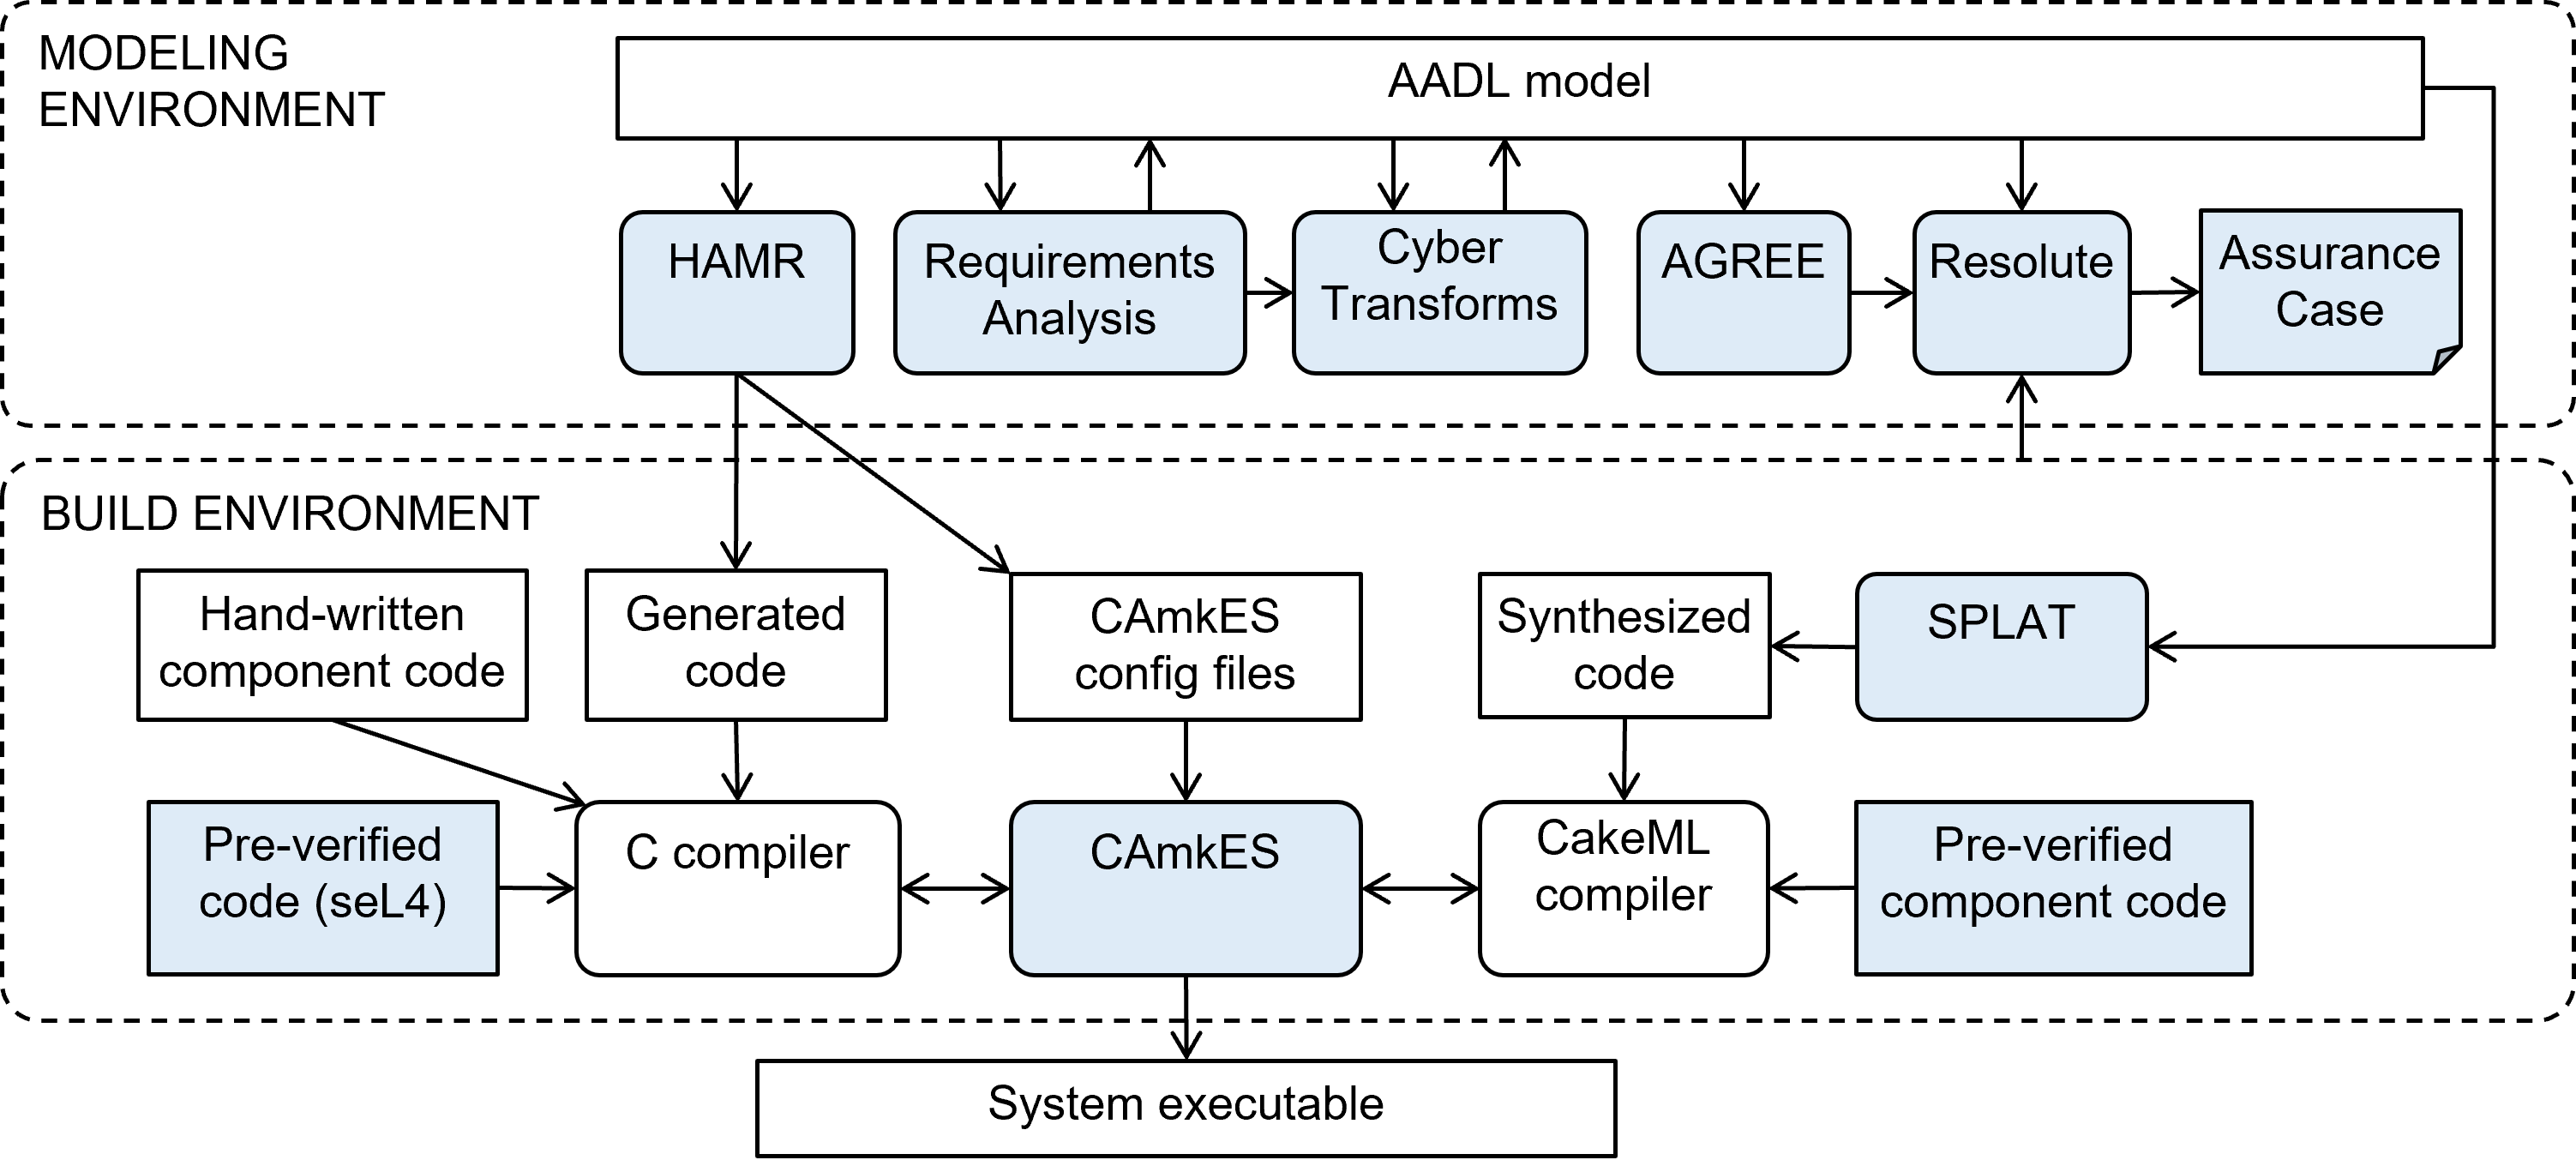
\includegraphics[width=\textwidth]{figs/briefcase-architecture.png}
	\caption{BriefCASE architecture. Tools and artifacts in the BriefCASE workflow are shown in blue.}
	\label{fig:briefcase-architecture} 
\end{figure}

\subsection{BriefCASE Architecture}

%	Cyber analysis / Req generation
BriefCASE provides access to two architecture analysis tools, GearCASE~\cite{gearcase2020} and DCRYPPS~\cite{dcrypps2019}, that analyze AADL models for potential cyber vulnerabilities and generate cyber requirements for mitigation. 
Systems engineers are presented with a requirements management interface for viewing the generated requirements and importing them into the model so they can be addressed.  
Some requirements can be formalized as assume-guarantee contracts, enabling formal verification. Such a requirement will be imported into the model with an associated formal contract.

%	Model transformation
To address a new cyber requirement, the architecture will need to be transformed in such a way as to harden the design against the vulnerability. BriefCASE provides an extendable library of model transformations for addressing common cyber vulnerabilities. 
The transformations are automated by the BriefCASE tool, resulting in a hardened model that is correct-by-construction. 
For example, the requirement that a component shall only receive well-formed messages can be satisfied by the insertion of a high-assurance filter. A BriefCASE transform wizard helps to configure the filter component properties, including the filter behavioral specification, which is represented as an assume-guarantee contract. BriefCASE then inserts a new filter component into the model, sets the component properties, and establishes the appropriate connections to source and destination components. The filter behavioral contract is also added to the model, enabling formal analysis of the model as well as providing the behavioral specification for a provably correct synthesis of the filter component implementation. 
The transformation also updates the assurance case with new evidential statements indicating how the associated goal has been satisfied, including the strategy used and context needed for assurance case evaluation.

%	Compositional analysis
The Assume Guarantee Reasoning Environment (AGREE)~\cite{compositional-analysis-agree}, is a compositional, assume-guarantee-style model checker for AADL models. AGREE attempts to prove properties about one layer of the architecture using properties allocated to subcomponents. The composition is performed in terms of assumptions and guarantees that are provided for each component.  
Once the system architecture has been modeled in AADL and component assume-guarantee contracts have been specified, the AGREE model checker is used to verify the consistency of these contracts.
AGREE results are automatically incorporated as evidence into the BriefCASE assurance case.

%	High-Assurance Component synthesis
%The correctness of the high-assurance components inserted by BriefCASE transformations means that each such component must meet its AGREE contract.
Each high-assurance component inserted by a BriefCASE transformation must conform to its AGREE contract. 
This obligation is addressed by formal synthesis, using the Semantic Properties of Language and Automata Theory (SPLAT) tool~\cite{case-models-2021}. SPLAT generates code to implement the AGREE contract and then proves that its implementation exactly preserves the meaning of the contract all the way down to the binary for the target platform.
%
SPLAT uses the HOL4 theorem proving system to implement the synthesis and prove its correctness relative to the contract. The synthesis targets a dialect of Standard ML called CakeML and uses CakeML’s fully verified compiler to render the final binary~\cite{cakeml}. 
%The SPLAT proof shows equivalence between the contract and the synthesized CakeML,
%The SPLAT proof shows that the synthesized CakeML conforms to the contract by 
%leveraging the existing CakeML compiler proof, and reasons about the perpetual re-execution of the code as scheduled in a real-time environment.

%	Infrastructure Code Generation
BriefCASE employs the High Assurance Modeling and Rapid engineering for embedded systems (HAMR) tool~\cite{hamr}, a multi-platform, multi-language AADL code generation framework. 
Using seL4~\cite{sel4-sosp09} as a foundation, HAMR enables AADL to be used as a model-based development and systems engineering framework for seL4-based applications~\cite{hamr-sel4}. 
The seL4 microkernel is a lightweight, fast, and secure operating system kernel. Its implementation is fully formally verified, from high-level security properties down to the binary level.

One of the primary objectives of HAMR is to support system builds that leverage seL4 separation and information flow guarantees to achieve the AADL-specified component isolation and inter-component communication needed for cyber-resiliency. 
%
For each AADL thread component, HAMR generates a thread code skeleton and APIs for communicating over the ports declared on the component. For components that are implemented manually, the developer fills out the thread skeleton with application code. 
HAMR generates component infrastructure and integration code implementing the semantics of AADL-compliant thread scheduling, thread dispatching, and port-based communication. 

The seL4 deployment uses the Component Architecture for microkernel-based Embedded Systems (CAmkES) code-generation framework to configure the microkernel. The HAMR-generated CAmkES directly encodes the AADL model’s component and communication topology and includes the AADL run-time infrastructure with its thread scheduling. HAMR leverages the existing seL4 domain scheduler to enforce time partitioning and provide static cyclic scheduling. 
As part of its code generation process, HAMR produces flow graphs reflecting the inter-component information flow at both the AADL architecture level and the CAmkES level for the seL4 deployment. Visual representations are provided for manual inspection, and SMT-based representations are generated for formal reasoning. The SMT-based representations are used to prove that 1) all AADL modeled flows are in the CAmkES configuration, and 2) no extraneous flows have been added. 


\subsection{Assurance Case Generation in BriefCASE}
\label{sec:resolute}

% Resolute
Each of the BriefCASE tools contribute to some aspect of high-assurance system development, and each emit evidence of correctness that can be used to substantiate cyber-resiliency assurance goals. Resolute~\cite{resolute2014} is used to evaluate this evidence and incorporate it into a system cyber-resiliency assurance case. 
%
%	Very high-level overview of Resolute
Resolute is a language and tool for embedding an assurance argument in an AADL system architecture model and evaluating the validity of the associated evidence. 
Because high-assurance products generally undergo certification at the system level, there is a natural mapping between a system design and the corresponding assurance argument. Resolute takes advantage of this alignment by enabling the specification of the assurance argument directly in an AADL \textit{annex}. The assurance case can then be instantiated and evaluated with elements specified in the model.

%	Maintaining cyber requirements in Resolute
BriefCASE projects contain a repository for cyber requirements. Imported requirements (e.g., those generated by GearCASE or DCRYPPS) are represented as assurance case goals to be satisfied. 
For example, a requirement that specifies that a target component shall only receive well-formed messages is imported as the Resolute \texttt{goal} depicted in Fig.~\ref{fig:resolute-requirement}a.  The goal is initially marked \texttt{undeveloped}.

\begin{figure}[h] 
	\centering 
	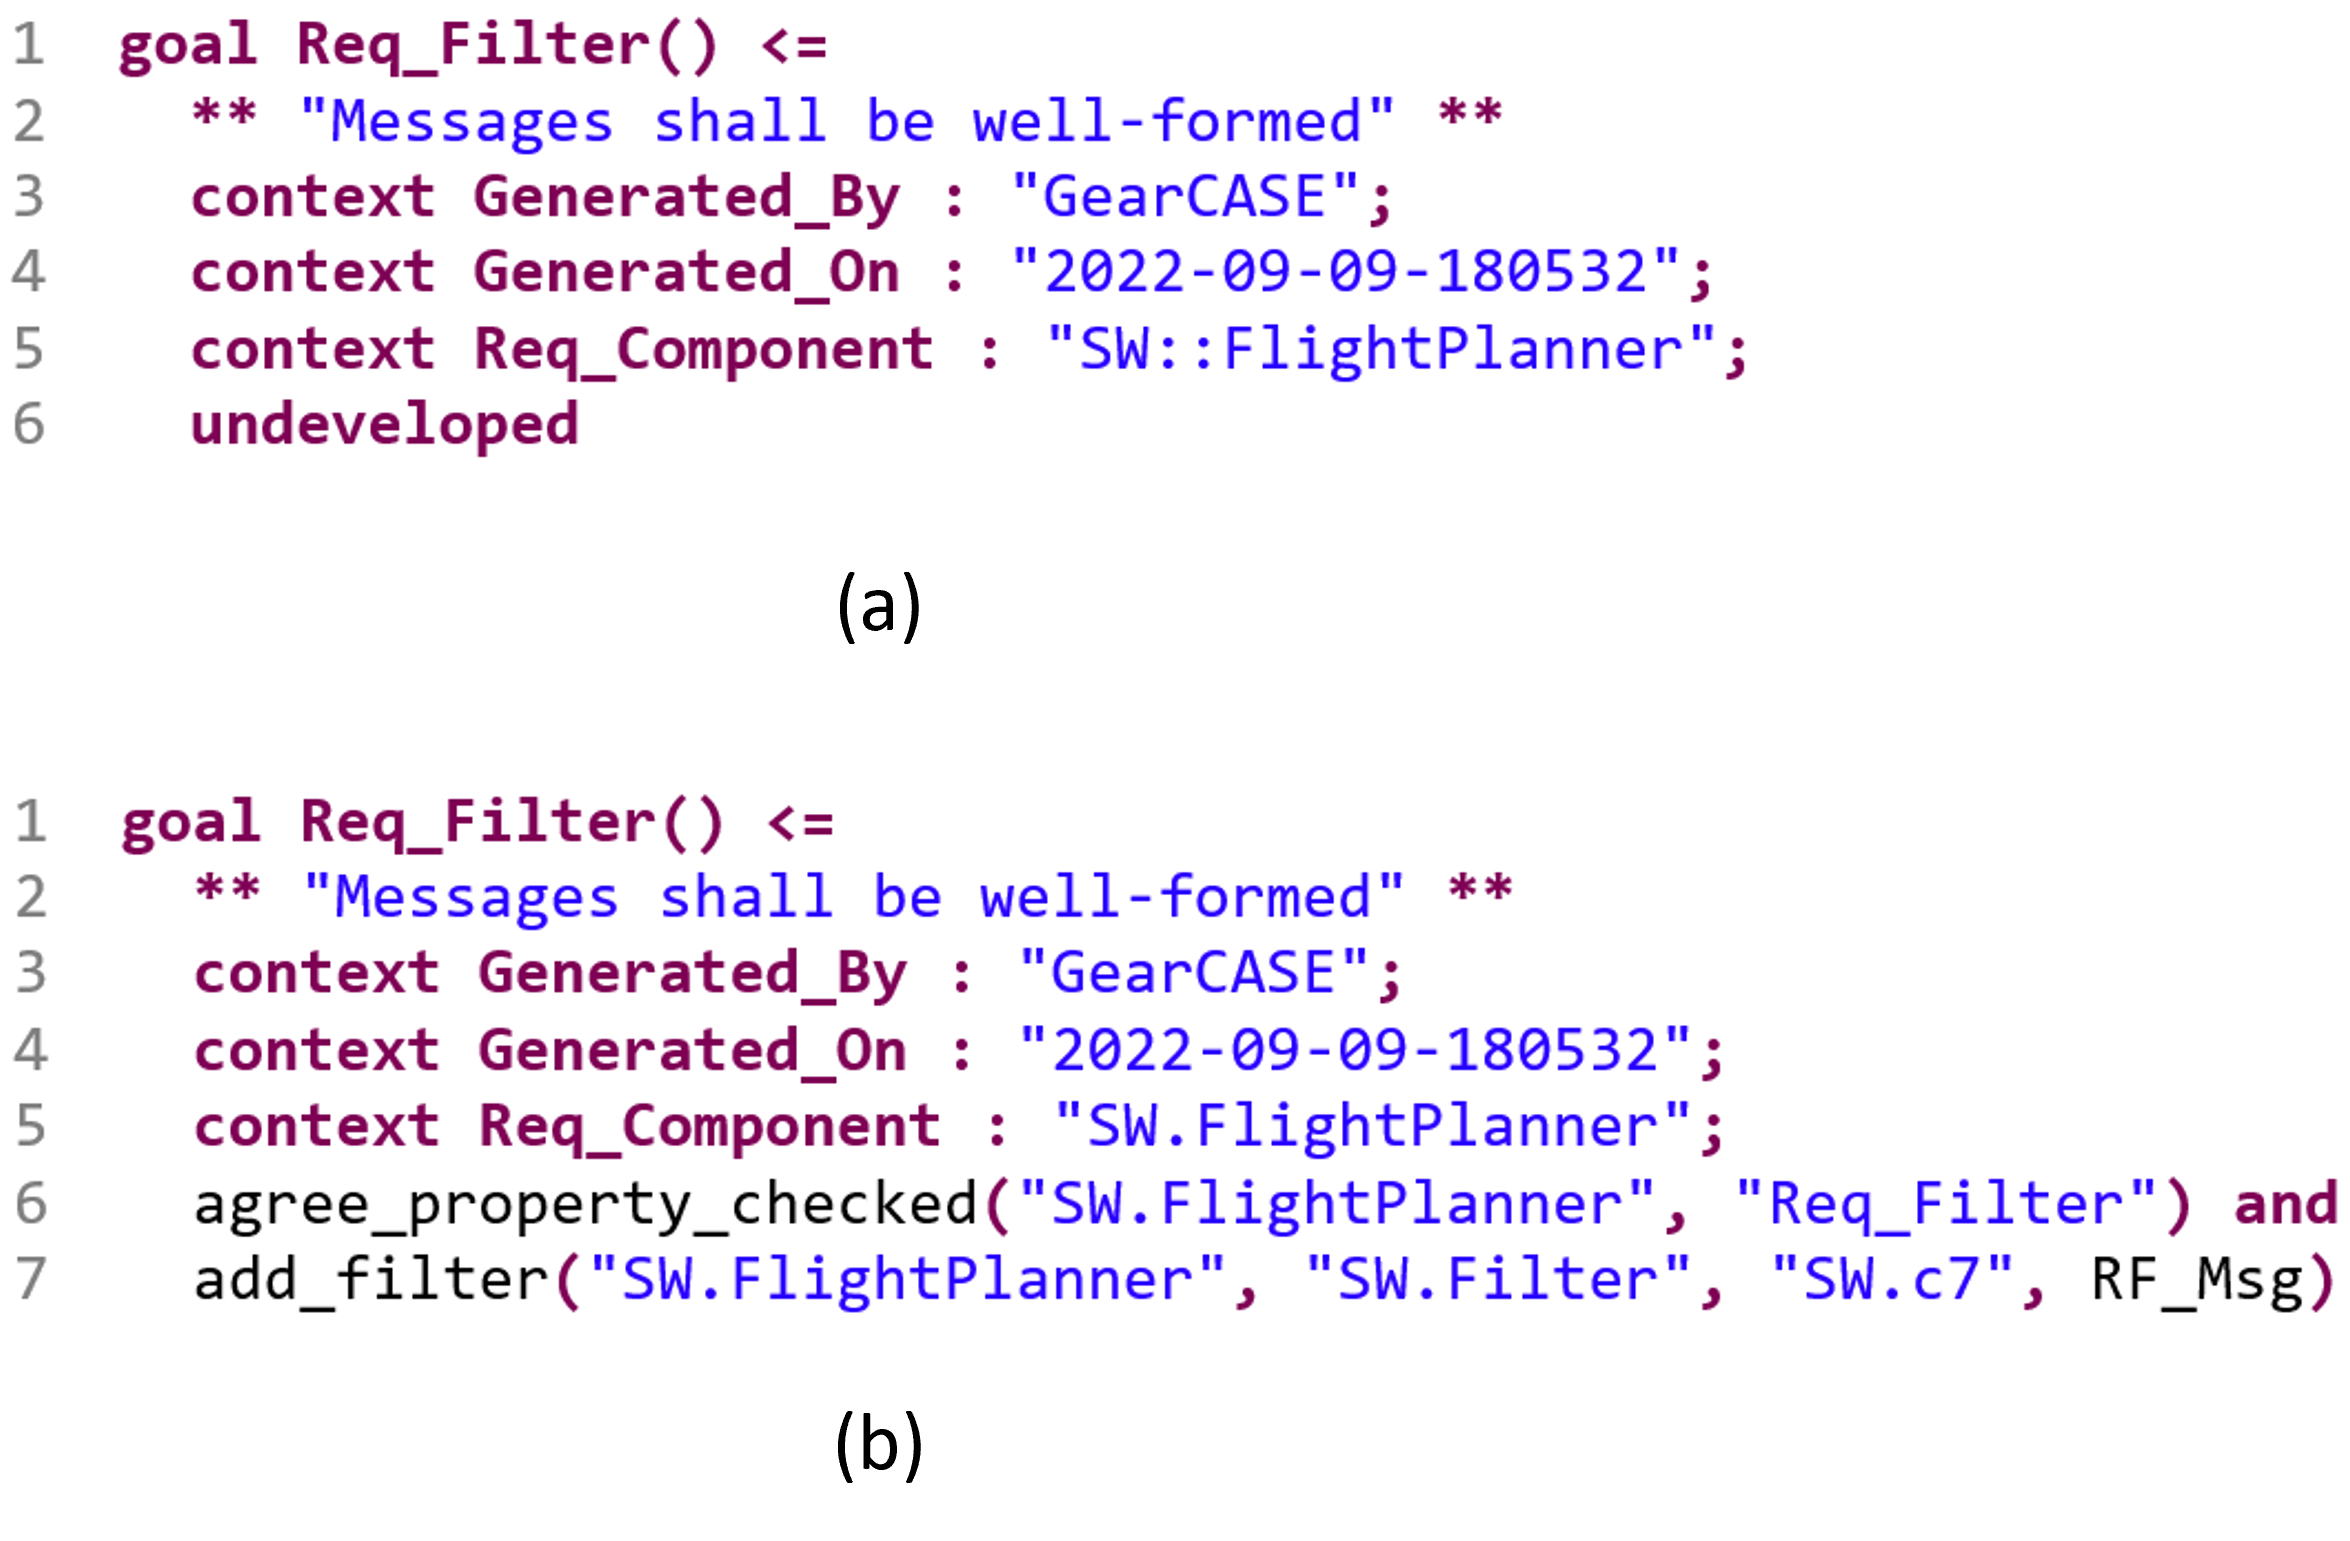
\includegraphics[width=\textwidth]{figs/resolute-requirement.png}
	\caption{(a) Cyber requirement imported as an \texttt{undeveloped} Resolute assurance goal.  (b) Updated goal with logical rules for determining whether goal is satisfied.}
	\label{fig:resolute-requirement} 
\end{figure}

%	Updating requirements with automated transform assurance library in BriefCASE
The well-formed message requirement can be mitigated by performing an automated model transformation for inserting a filter. Each transformation has an associated assurance pattern that describes a strategy for determining from the model whether the requirement has been satisfied (see Section~\ref{sec:requirements-satisfied-in-model}).  
These evidential statements are added to the goal as the design is updated to address the requirement, as shown in Fig.~\ref{fig:resolute-requirement}b.  For the insertion of a filter, Resolute must now check that AGREE formal analysis passes (line 6) and the filter was added correctly to the model (line 7).  The \texttt{agree\_property\_checked()} and \texttt{add\_filter()} function definitions are included with the built-in BriefCASE assurance pattern library and contain additional statements that instruct Resolute on how to determine the validity of the claims. 
Subsequent changes to the model that invalidate any of the assurance claims can then be detected and corrected.  

%	Specifying external evidence in Resolute
Resolute has recently been updated to enable evaluation of artifacts external to the modeling workspace. BriefCASE includes an Artifact Management tool for specifying how Resolute should parse documents with specific formats (such as test results, review forms, etc.) to determine whether they support specific assurance claims.  For each type of document, users can specify a regular expression that will be matched against the document contents, such that a correct match indicates the validity of the evidence in supporting a specific claim.

%	BriefCASE assurance pattern in Resolute
The assurance patterns presented in our previous work (see~\cite{resolute-destion}) primarily focused on design assurance; that is, correctness of the architecture model.  With recent updates to BriefCASE and Resolute, we have since expanded the patterns into a comprehensive cyber-resiliency assurance argument covering architecture design, code synthesis, and system build.  The assurance patterns (described in the next section) are formalized in Resolute and included with BriefCASE.
